
\chapter{A note on the the theory of rent and urban economic development, August 20 2022}\section{initial notes}

This document describer the link between housing cost, rent theory, and urban prosperity. The analysis has important implications for Ontario Housing Policy and Canadian economic development

The key idea is that cites are productive and we want to understand how the surplus wealth produced by cities is distributed.  It turns out that ownership of land determines  who gets the surplus. Land is a natural resource- no one creates it. The share or production that goes to landowners is called "rent." To  understand what is happening in our cities we need a basic grasp of  rent theory, first developed by David Ricardo. 

We first very briefly review the familiar supply and demand graph. We then show how Ricardian rent theory is implicit in the model when we apply it to  the ownership of agricultural land. That allows us to show how the basic model of modern urban economic is a variant of Ricardo's model and can be used to approach the question of distribution. Finally we 

\section{A preamble}
Ricardo provided an explanation for the wealth and power of the landowning classes in Britain. Ricardo's theory remains one of the basic tools of modern economics, appearing in every first year economics course as consumer and producer surplus, in urban theory and the classic urban rent profile and in institutional theory as  "rent seeking."

Straightforward application of Ricardo's insight using simple supply and demand curves allows us to understand the current housing crisis and the national productivity crisis. It also points the way to a strategy that can solve the housing crisis, make Canadians better off and increase the productivity of the Canadian economy.

  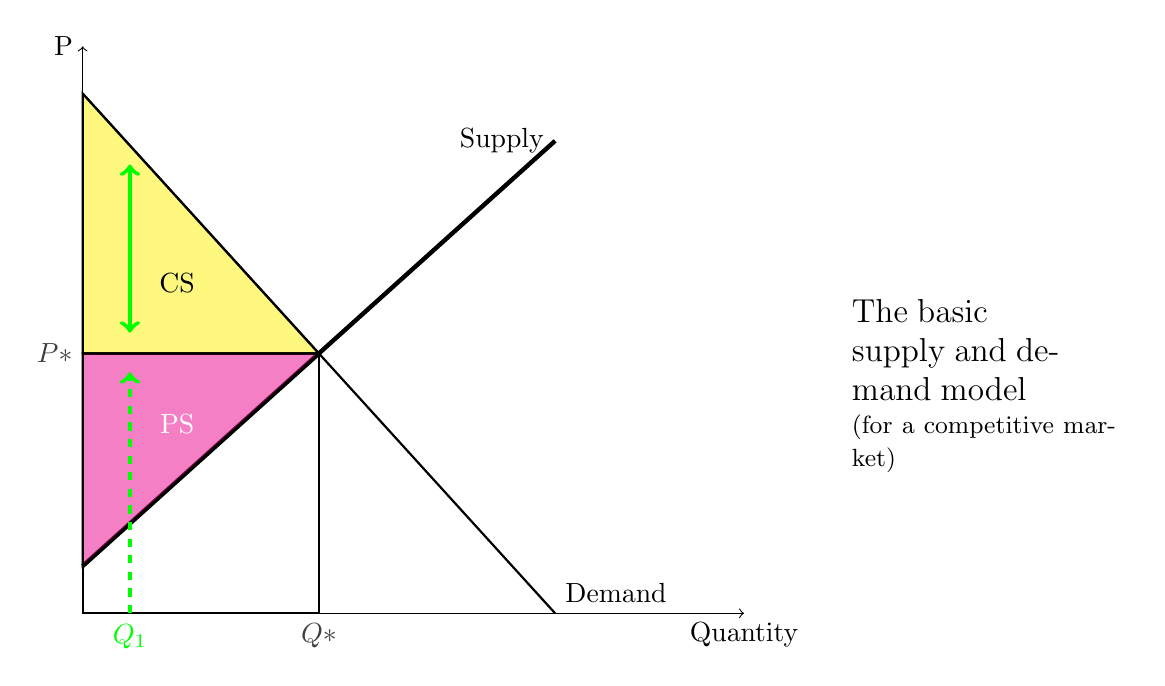
\begin{tikzpicture}[domain=0:2,scale=1.2]        %NINE panesl Top lcr M lcr Blcr
%%%%%%%%%%% 								               TOP%%%     
 %	 \begin{scope}[scale=.6, shift={(6,20.5)}]  % Tr : features of S and D 
			%  \draw [gray] (0,0) grid (7,7);
		\draw [<->] (0,6)node[left]{P} -- (0,0) -- (7,0)node[below]{Quantity};
  
		\draw [thick] (0,5.5) -- (5,0)node[above right]{Demand};
	%	\node at (5,0)[below]{$Q_{max}$};
		\draw [ultra thick] (0,.5) -- (5,5)node[left]{Supply};
				 
		 \draw [thick, fill opacity=0.75] % fill=yellow,
		 		(0,0) -- (0,2.75) node[left]{$P*$}--(2.5, 2.75) --(2.5, 0)node[below]{$Q*$} -- cycle;
 		\draw [thick, fill=yellow, fill opacity=0.5]  
				(0,5.5) -- (0,2.75) --(2.5, 2.75) -- cycle;
 		\draw [thick, fill=magenta, fill opacity=0.5]  
				(0,.5) -- (0,2.75) --(2.5, 2.75) -- cycle;
				
 		% \node at (1.5,1)  (a) [red] {VC};
		 \node at (1,2) (b) [white] {PS};
		  \node at (1,3.5) (b) [black] {CS};

	\draw [ultra thick, green, <->] (.5, 4.75) -- (.5, 2.97);
	\draw [dashed, ultra thick, green, ->] (.5, 0)node[below]{$Q_1$} -- (.5, 2.55);


  \begin{scope}[scale=.6, shift={(10,0)}] 
		    \node at (6,4) (b) [black, text width=3.5cm] {\large The basic \\supply and demand model\\ {\small (for a competitive market)}};
\end{scope}		    
\end{tikzpicture}
\section{Basic Supply and Demand}
We can begin with the basic supply and demand graph, although the graph was not invented in Ricardo's time. In this figure, the height of the demand curve at each quantity represents how much buyers will pay for  one more unit of whatever is being sold in this market. The height of the supply curve is the cost of producing one more unit. Producers won't want to sell any units that cost more than they are being paid.

To read the graph, we can pick a price, and read horizontally to the demand curve to `predict' how many consumers  want to buy at that price, and across  the supply curve to find out how many producers want to sell. If they don't agree on a quantity to transact, we have a problem. They will agree on quantity at the price $P*$ where the curves cross, however. As a result we might expect to see actual  prices bouncing around this value.

Notice that if there are a lot of buyers, some of they may value the product more  that the price they pay. The green arrow in the yellow area of the figure is the amount of `consumer surplus value' received by whoever bought unit $Q_1$.

%Overall, the supply and demand graph  is a remarkably simple  model that lets us think clearly  the behaviour of hundreds, or even millions, of two different kinds of people, the buyers and sellers, when they interact. It finds a combination of price and quantity that is likely to be reasonably stable, and it can be applied to all kinds of markets. 

\section{Ricardo's problem}
Ricardo was analyzing the agricultural sector which depended on land. He wanted to explain how the surplus produced by the land was share between landowners and labour. His analyses leave out consumers, and the producers are the landowners, because they owned what Marx would later call ``the means of production''. 

We can adapt the supply and demand  model to describe what Ricardo discovered,  The height of the supply curve. becomes the labour cost of producing  `corn' (we call it wheat now) on each plot of land from best on the left to the worst on the right. Naturally cost in labour rises as we move to less productive. The supply curve now shows the rising cost as more land is planted.

Landowners didn't actually farm, and they didn't usually hire workers to  farm the way that an industrial. capitalist did. They  rented plots land to peasant farmers. Their problem came down to figuring out how much rent they could charge for each plot of land they rented out. Maximizing their rent  income meant minimizing the share of the surplus that the peasants got to keep. 

Landowner and peasant knew roughly what  price would be paid for `corn' (we call it wheat now) when it was produced, how much corn a particular plot would produce, and how much work it would take to produce that corn. Although the rent-setting process was probably quite different, we can imagine the peasant knowing the maximum he would bid to farm a particular lot.  We can imagine the peasant and the landlord negotiating over the rent. 

Since land was scarce and peasants were numerous, the landlord generally had the upper hand and could squeeze out something close to the maximum rent. After the black death there were fewer peasants  and they were able to negotiate lower rents.


Looking ahead, the everyone would have some sense of the  price of corn. No one expects their decision to affect that future price, we don't need the demand curve - in the figure we just rotate it down until it is flat. 

The problem was to decide how much land to plant. The cost price  growing corn on the best land was very low, but but it would increase as cultivation extended onto lower quality land. 



Since the landowner has a price in mine we don't need the demand curve - we just rotate it down until it is flat. 

\begin{figure}[htbp]
\begin{center}

  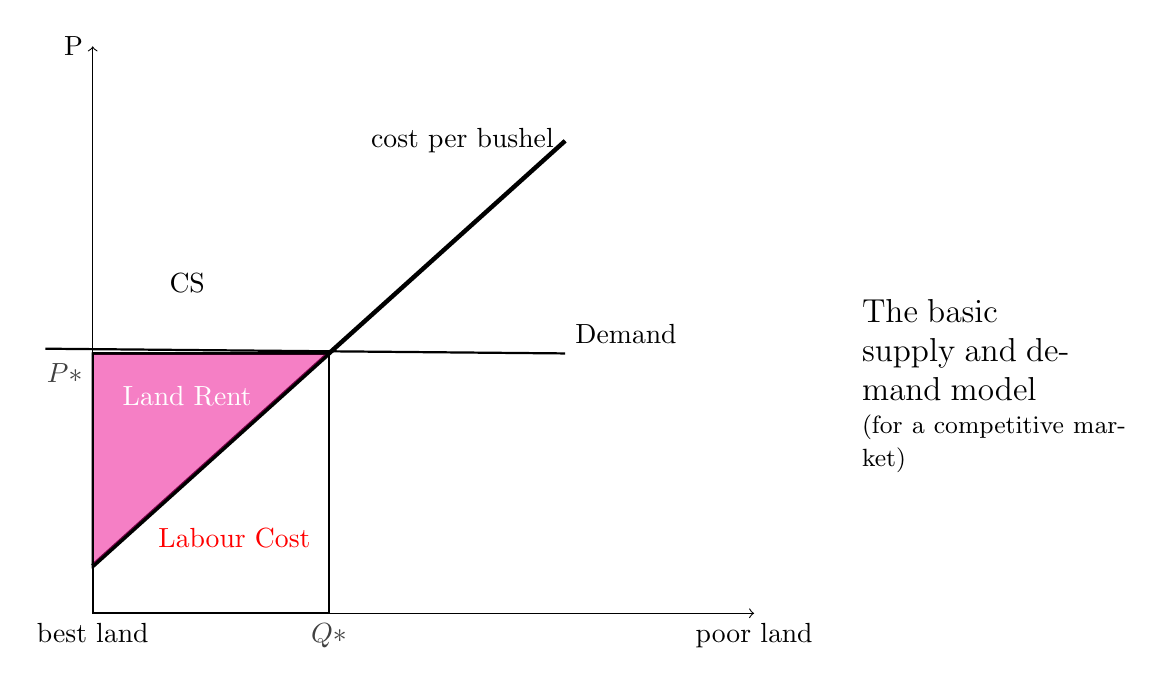
\begin{tikzpicture}[domain=0:2,scale=1.2]        %NINE panesl Top lcr M lcr Blcr
%%%%%%%%%%% 								               TOP%%%     
 %	 \begin{scope}[scale=.6, shift={(6,20.5)}]  % Tr : features of S and D 
			%  \draw [gray] (0,0) grid (7,7);
		\draw [<->] (0,6)node[left]{P} -- (0,0)node[below]{best land} -- (7,0)node[below]{poor land};
  
		\draw [thick] (-.5,2.8) -- (5,2.75)node[above right]{Demand};
		%\node at (5,0)[below]{$Q_{max}$};
		\draw [ultra thick] (0,.5) -- (5,5)node[left]{cost per bushel};
				 
		 \draw [thick, fill opacity=0.75] % fill=yellow,
		 		(0,0) -- (0,2.75) node[below left]{$P*$}--(2.5, 2.75) --(2.5, 0)node[below]{$Q*$} -- cycle;
 	%	\draw [thick, fill=yellow, fill opacity=0.5]  
				(0,5.5) -- (0,2.75) --(2.5, 2.75) -- cycle;
 		\draw [thick, fill=magenta, fill opacity=0.5]  
				(0,.5) -- (0,2.75) --(2.5, 2.75) -- cycle;
				
 		 \node at (1.5,.8)  (a) [red] {Labour Cost};
		 \node at (1,2.3) (b) [white] {Land Rent};
		  \node at (1,3.5) (b) [black] {CS};

	%\draw [thick,dashed] (.5,7) -- (.5,0)node[below]{$Q_{low}$};


  \begin{scope}[scale=.6, shift={(10,0)}] 
		    \node at (6,4) (b) [black, text width=3.5cm] {\large The basic \\supply and demand model\\ {\small (for a competitive market)}};
\end{scope}		    
\end{tikzpicture}
\caption{Ricardo's Figure}
\label{Fig:Ricardo'sFigure}
\end{center}
\end{figure}
